
  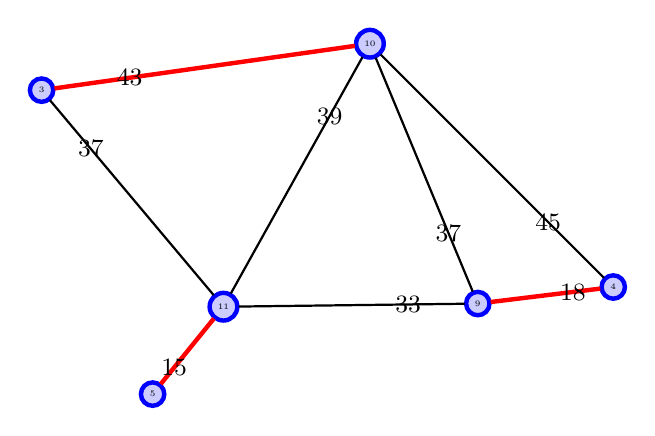
\begin{tikzpicture}[scale=10, ultra thick, node_style/.style={circle,draw=blue,fill=blue!20!,scale=0.6,font=\tiny},terminal_style/.style={circle,draw=red,fill=white,scale=0.6,font=\tiny},edge_style/.style={draw=black, thick,font=\small}, selected_edge_style/.style={draw=red, ultra thick,font=\small}, selected_edge_style-2/.style={draw=purple, ultra thick,font=\small}]
      \draw
        (0.191, 0.669) node[node_style] (3){3}
        (0.917, 0.419) node[node_style] (4){4}
        (0.332, 0.283) node[node_style] (5){5}
        (0.745, 0.398) node[node_style] (9){9}
        (0.608, 0.728) node[node_style] (10){10}
        (0.422, 0.394) node[node_style] (11){11};
      \begin{scope}[-]
        \draw[edge_style] (3) to node[near start] {37} (11);
        \draw[selected_edge_style] (3) to node[near start] {43} (10);
        \draw[edge_style] (4) to node[near start] {45} (10);
        \draw[selected_edge_style] (4) to node[near start] {18} (9);
        \draw[selected_edge_style] (5) to node[near start] {15} (11);
        \draw[edge_style] (9) to node[near start] {37} (10);
        \draw[edge_style] (9) to node[near start] {33} (11);
        \draw[edge_style] (10) to node[near start] {39} (11);
      \end{scope}
    \end{tikzpicture}
